\documentclass[a4paper]{report}
\usepackage{xcolor}
\usepackage{graphicx}
\usepackage{url}
\usepackage{hyperref}
\usepackage{setspace}
\usepackage[sort,nocompress]{cite}
\usepackage[titletoc]{appendix}
\begin{document}


\newcommand{\fig}[4]{

\begin{figure} 
    \centering
    \includegraphics[scale = #4]{#1}
    \caption{#2}
    \label{#3}
\end{figure}


}
\newcommand{\figh}[4]{

\begin{figure} [ht!]
    \centering
    \includegraphics[scale = #4]{#1}
    \caption{#2}
    \label{#3}
\end{figure}


}
%%1964

\begin{titlepage}
   \begin{center}
       \vspace*{1cm}
 
       \LARGE\textbf{Making Git Accessible For Children}
 
       \vspace{0.5cm}
        Third Year Project
 
       \vspace{1.5cm}
 
       \textbf{Samuel Da Costa}
 
       \vfill
 
 	  
       BSc (Hons) in Computer Science and Mathematics\\
       Supervisor: Caroline Jay 
 
       \vspace{0.8cm}
 
       
\includegraphics[width=0.4\textwidth]{figures/university}
 	\normalsize
 
   \end{center}
\end{titlepage}



\begin{abstract}
This report discusses a project aimed to bring version-control to children through a simplified interface to the Git version-control system. An argument that such software is needed will be presented, and the design and implementation of the software discussed. This will include a discussion of how the system was split into distinct components and the individual challenges involved in implementing these components. We will discuss the testing strategy, both in terms of automated testing and the use of focus groups to obtain real user feedback. Finally, this report reflects on the achievements of the project and comments on decisions that would be made differently if the project restarted.
\end{abstract}

\renewcommand{\abstractname}{Acknowledgements}
\begin{abstract}
I would like to express my gratitude to Caroline Jay, Robert Haines and my third year tutor group for their continued support from the very beginning of my project and for their insightful comments and feedback throughout.

\end{abstract}

\tableofcontents

\chapter{Introduction}

In England and Wales, the percentage of students choosing to study a GCSE in Computer Science rose by 50\% from 2015 to 2016 and continued to rise between 2016 and 2017. This is according to official statistics published by Ofqual  \cite{ofqual}.

Moreover, the UK government has introduced simple programming to children as young as five years old \cite{primarycoding}, suggesting that more and more young people are beginning to produce code.

This project does not aim to convince the reader that toddlers require a source-control system. However, students studying their GCSEs and A-Levels in Computer Science often produce non-trivial amounts of code, the need for complete backups and version control become more apparent.

In the field of computer science, this is a solved problem. The \emph{Git} \cite{git} source-control system solves all these problems. Git provides means of easily keeping backups, keeping track of versions and the ability to roll back to an old version easily.

Of course, using Git comes with its challenges. To use it effectively requires practice and an understanding of its low-level commands which can be daunting to new users.

This project aims to strike a balance between the complexity of the system and the needs of younger users. To take advantage of such a feature-rich version-control system and to provide an interface to it which can be understood and used even by children.

The emphasis of this interface is on the concept of \emph{version-control} rather than Git specifically. Abstracting and automating the internals of Git to allow the user to concentrate on the higher level concepts such as, ``rolling back," and, ``saving a new version".

\section{Background on Git}

This section briefly describes some of the main advantages of Git and introduce some relevant terminology. 

As previously mentioned Git allows for straightforward backups. In practice, this means the existence of a remote server which also holds a copy of the user's code. When the user wishes to back up their code, they create what is known as a \texttt{commit} object. Such an object contains a subset of the files in the directory that the user has edited since the last commit, as well as metadata such as the date, author e.t.c. Importantly, the metadata contains a pointer to the commit that was created before it. The resulting structure then forms a graph of project history.

At any point in the future, the user now can reset the project to the state stored in any \texttt{commit}. Given these objects, Git handles backups by providing commands that allow secure storage of the objects on a remote server (referred to as \emph{pushing} to the remote server). 

Sharing of projects across devices now becomes simple. The user on a different device makes a copy of the project from the remote server (referred to as \emph{cloning}). They are then free to create commits and to push them to the remote server, and to pull down commits created by others.

In practice, however, the use of these commands can often be fiddly for new users.  The following is merely the author's opinion and should not be interpreted as a statement of concrete fact. This being said, it seems clear that Git's main complexity comes from the fact that any piece of code could be in one of many places. It could exist in a stash, in the working directory, in the staging area, in a commit on the remote e.t.c.

Users are required to know about all these different areas and how they interact. When they inevitably make a mistake, usually this results in an error which is very difficult to read and interpret. 

With this in mind, the first goal of this project becomes clear. To abstract away as many of these different locations as possible. We will see that the project presents the user with only two areas: the remote version, and their local version.

\section{Project Goals}\label{sec:projectgoals}

At the outset of the project, there were three main objectives, from which all other aims extend. These are as follows.\\

\subsection{Objective 1} 

The first objective was to produce a user interface which should be useable by anybody over the age of thirteen years old. This interface should enable interaction with an underlying Git repository at a very high level of abstraction. \emph{Note:} The GUI is not aiming to \emph{teach} the user about Git, or even about version-control. The idea, is that given a brief introduction to the concept of version-control, that the user should be able to use the system.

To define specific use-cases that the GUI should support, it was essential to consider the behavior of Git users. A questionnaire was circulated to adult users who already use Git to determine which operations are considered most useful, and which are most challenging to use. 

For the project, we'd aim to support the most useful operations, for those useful yet challenging tasks the aim was to support them but possibly in a simplified form. A prime example of this is branching, 96\% of respondents indicated branching was important to their workflow, but only 66\% found branching to be an easy task. Therefore, a simplified branching procedure is used whereby branches are automatically created and managed as the user navigates back and forth through the commit history.

Furthermore, the survey indicated that only 7.4\%  considered the setting up of SSH keys to be easy, with a further 77\% saying they always needed to look up instructions for how to do so. Therefore this project aims to handle all SSH authentication automatically.

The supported use-cases were also heavily influenced by studying the national curriculum for Computing in England for the target age group \ref{primarycoding}. It reveals that students are not required to work in teams or work on the same code. Because of this, the GUI concentrated on a single user's needs, for example, the branching structure described above is ill-suited to a repository with multiple collaborators but provides a much simpler user experience for the single user \footnote{The system does fully support multiple users interacting with a repository. We simply optimise the GUI for one user, possibly on multiple machines since this is the most likely scenario. }.

What follows is the list of use cases the project initially aimed to fulfil. The use case highlighted in red was removed since it was judged to add needless complexity.

\begin{itemize}
\item Ability to login on any machine with the software installed and see a list of projects.
\item Ability to open any of these projects locally just with a click.
\item New commits should appear on other machines logged into the same user account without the need for the user to perform manual steps.
\item Ability to jump back and forwards through the project history.
\item \color{red}Ability to choose which files to add to a commit \color{black}
\end{itemize}


\subsection{Objective 2} 

The second objective was less tangible and to produce a system that is scalable, well tested and robust enough for use by inexperienced users. In practice, this last part implies that the system should be able to automatically detect and correct issues with the underlying Git repository which would usually need to be manually corrected.

Scalability is an essential part of this project. Consider the case that the project is wildly successful and has many users beginning to use it. The result would be many repositories needing storage on remote servers. One of the key aims of the project is to build a system that allows adding more remote machines to the pool of available resources and that the system automatically begins using these multiple servers.

\subsection{Objective 3}

Finally,  the project's third objective was to introduce the software to children and gather feedback about how useful it would be to them. This objective is fundamental; without user feedback and appraisal there is no way of knowing if the software is fit for purpose.

By the end of the project, two feedback sessions were conducted with school children during a Computer Science lesson at their school. We'll discuss their feedback and the approach to the sessions in Section \ref{sec:user-testing}.

 \chapter{Technical Design}

This chapter aims to describe and explain the system's overall architecture. To explore potential performance bottlenecks and their solutions, as well as discussing the roles of the individual components that make up the final solution. This chapter does not discuss the implementation details, but rather give a high-level view of the \emph{why} rather than the \emph{how}. It is relevant to mention that the system as a whole has been informally dubbed `littlegit', a name used throughout this report.

\section{Other work in this area}

So-called \emph{Git GUIs} (graphical user interfaces to Git) have existed for almost as long as Git itself. Notably, Git itself comes with two visual tools, \textbf{gitk} and \textbf{git-gui}. The former is used mainly for viewing the commit history, and the latter's main function is to create commits \cite{gitguis}. However, these tools provide minimal functionality beyond a graphical way of invoking git commands. There is very little automation, and a reasonable knowledge of Git is still very much required. Furthermore, they provide no help with the generation of SSH keys, which are used by Git for authentication.

At the time of writing the most comparable system to that which this project aims to create belongs to Atlassian. The user can manage remote repositories, clone them to their local machine, view history and interact with the repository in many complex ways through the desktop application \emph{SourceTree}. The most noticeable feature here is the management of remote repositories from within the same application. However, here too is where the automation stops. There is little to no help with the resolving of conflicts, SSH key setup is still a manual process, and most importantly, errors from git are often directly passed onto the user with no attempt to resolve the issue for them. Figure \ref{fig:sourcetree_issue} is an example of this.

\fig{figures/sourcetree_issue.png}{An example of SourceTree passing errors on to the user.}{fig:sourcetree_issue}{0.3}

The project, therefore, aims to build upon the positive features of SourceTree and the Atlassian ecosystem, adding more abstraction and automation in the hopes of achieving a much simpler user experience.

\section{Technical Overview}

First, we present a very high-level description of the system as a whole, before exploring its components and their roles. Figure \ref{fig:highlevel} shows a high-level representation of the system. The desktop GUI is the application the end user installs and uses to manipulate their repositories.

\begin{figure} 
    \centering
    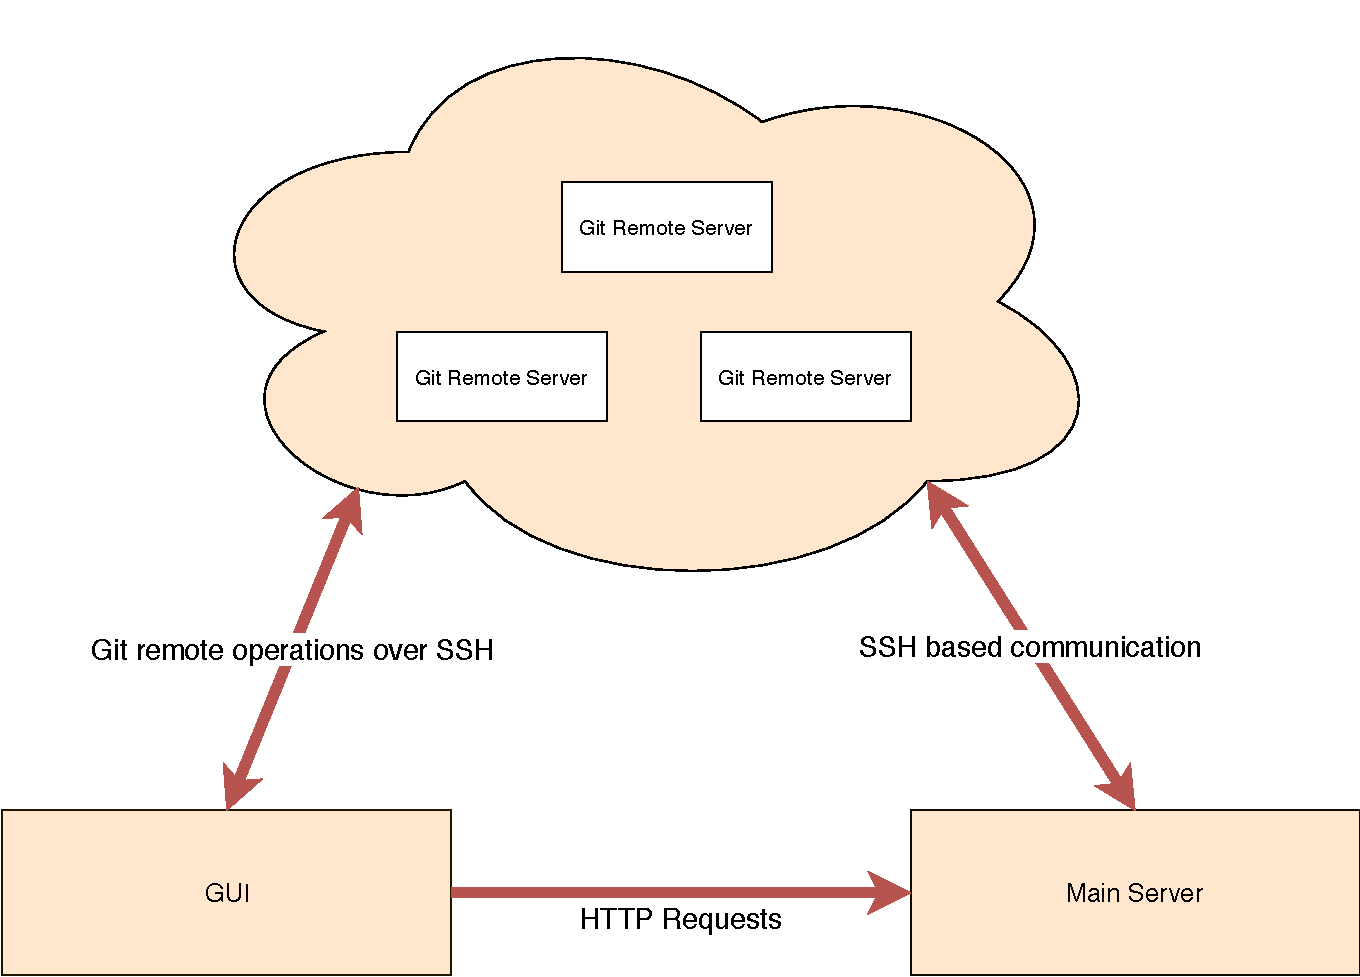
\includegraphics[scale = 0.5]{figures/highlevel.pdf}
    \caption{A high level representation of the architecture of the system. }
    \label{fig:highlevel}
\end{figure}

The Git servers are the machines that host these remote repositories. These are distinct from the main server which does \emph{not} host repositories but manages the system as a whole.

\subsection{Git Servers and the Main server}

The reader may ask whether this infrastructure is needed. There already exist many hosting services for Git repositories. GitHub, Gitlab and Bitbucket to name a few. However, using these limits our ability to automate as much as possible. To be able to perform tasks such as setting up SSH keys for the user we must have complete control over the backend infrastructure. 

Furthermore, this control allows for easy integration of new features in future. For example, we could introduce a new type of user such as a teacher who could have access to multiple repositories. To introduce such a role while relying on the stability of a third party service would be much more difficult.

Figure \ref{fig:highlevel} shows multiple Git servers; this demands some explanation. A reasonable question to ask is why is one not sufficient? The second objective of this project is to produce a scalable system. We must ask ourselves what happens if we start to get more users, creating more repositories. One server soon runs out of space. 

Moreover, our system is likely to slow when one Git server alone has multiple other machines communicating with it simultaneously. For this reason, we spread the load of Git repositories over multiple machines. A future goal of this project is to have machines hosted in different regions around the world, and assign their repositories based on the location of users to make the system as efficient as possible.

Of course, having multiple servers hosting Git repositories presents its own set of challenges. For a user's machine to be able to communicate with a Git server, we must register its public SSH key on all the Git servers that host the user's repositories. One of the responsibilities of the main server is precisely this. To manage SSH keys, ensuring the right ones exist on the correct machines, which becomes more complicated when we realise that an SSH key is associated to a machine, not a user and that a user may work on multiple machines necessitating multiple keys.

The main server provides API endpoints for the GUI to use to handle all user authentication, create new repositories and importantly, to register new SSH keys.

\subsection{Desktop GUI}

The GUI is the desktop application the end user interacts with and uses. Its primary responsibilities are to allow the user to manipulate the Git repository and visually display its current state. It also is responsible for the aforementioned automation of Git and resolving of issues.

\begin{figure} 
    \centering
    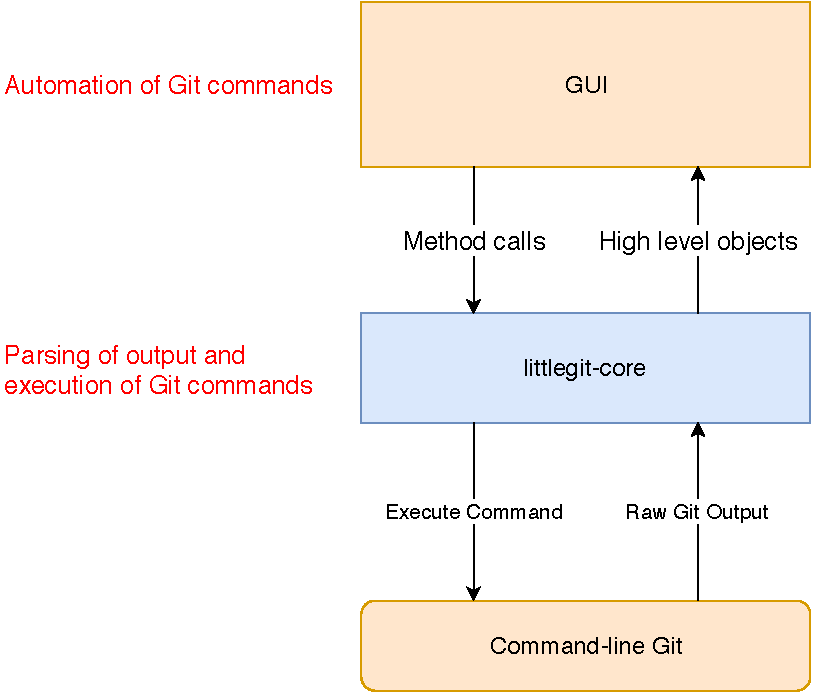
\includegraphics[scale = 0.5]{figures/gui-core.pdf}
    \caption{A representation of the interaction between the GUI and the littlegit-core }
    \label{fig:gui-layers}
\end{figure}
\subsubsection{ Low-level git library}

At this stage, it's prudent to mention the way both the GUI and the main server interact with Git itself. This interaction happens through the medium of a library called the \textbf{littlegit-core} written for this system and included by the GUI and server as a dependency. It serves as a wrapper around the Git command line allowing interaction from a high-level language (discussed further in Chapter 3) with the Git binary. The littlegit-core is responsible for executing Git commands and parsing the output into useful high-level objects as Figure \ref{fig:gui-layers} describes. 

\section{UI Design}
 
Early in the project, the interfaces of other Git GUIs were examined, exploring their strengths, weaknesses and most importantly, their common traits. The findings of this research are discussed here as well as a discussion of how the results impacted the design of this project's user interface.

The three main applications researched are the application SourceTree \cite{sourcetree} (mentioned earlier), GitKraken\cite{gitkraken} and GitK\cite{gitk}. Figures \ref{screenshot:sourcetree}, \ref{screenshot:gitkraken} and \ref{screenshot:gitk} show a screenshots of their main interfaces.

\fig{figures/sourcetree.png}{A screenshot of the main interface of the application SourceTree.}{screenshot:sourcetree}{0.32}

\fig{figures/gitkraken.png}{A screenshot of the main interface of the application GitKraken.}{screenshot:gitkraken}{0.25}

\fig{figures/gitk.png}{A screenshot of the main interface of the application GitK.}{screenshot:gitk}{0.3}

The first thing to note in looking at the interfaces is the common element being the Git graph. Though each has a different style and displays the information differently, the graphs are all prominent features of each interface. The decision was made to emulate the overall style in littlegit. The vertical graph, new commits on top with older commits in descending order below them. The reasoning here is that the Git history portrayed in this way conveys all necessary information, but is easy to present a simplified version (as was needed for littlegit) by merely omitting some of the information surrounding it.

However, other options were considered, Figure \ref{fig:horizontal-graph} shows an early design for an alternative graph which scrolls horizontally. The idea was to emulate a timeline to help visualise the repository as being a series of snapshots of the code, allowing the user to navigate backwards and forwards along it. This idea however soon proved impractical, visually representing branches in this model becomes messy and complicated, especially for more complex repositories. Furthermore, according to user testing \cite{horizontalScrolling}, users dislike horizontal scrolling.

Returning to our discussion of the other applications, the graphs of both SourceTree and GitK are relatively cramped. A large amount of information in very close proximity, this is especially true of GitK. On the other hand, GitKraken takes much more space to display the same information, a feature it was important for littlegit to emulate to ensure the data is clear and easy to understand.


\fig{figures/horizontal-graph.pdf}{An early design for the Git graph using horizontal scrolling.}{fig:horizontal-graph}{0.5}

Moreover, all three applications have lots of buttons and menus. After studying these controls, it became clear that in a system that aims to automate as much as possible the vast majority of the options were unneeded. For example, SourceTree has three separate buttons for pushing, pulling and fetching. The question littlegit asks is why? If there is something to push to the server, why not just do it on the users' behalf, and if there are no new changes on the server to be pulled, then why present the user with the option? This lead to the decision to use a popup dialogue to indicate when the user's local version is behind the server, giving them the option to update without the need to clutter the primary interface with the option.

Since this automation is taking place, it seems prudent to explicitly describe the Git workflow littlegit aims to present. The workflow is built around the commit, creating commits should drive everything else. Creating a commit causes changes to be pushed to the server, and the arrival of new commits on the server should cause the application to update the repository accordingly. Branches in this workflow are much less significant than int other workflows, only being used by littlegit internally when needed. Looking back at SourceTree especially, it is unclear how to create a new commit in its interface. Since commits drive littlegit, it was imperative to avoid this.

Furthermore, by looking at GitKraken and SourceTree in particular, the reader may also notice that many of the buttons on their left toolbars are merely the names of branches. In regular use clicking on them allows the user to check out these branches. Both applications also allow for using the graph to navigate between branches, allowing the user to click on the branch they wish to check out. 

Use of the graph for navigation seemed an efficient and intuitive approach. With littlegit we aimed to expand this functionality, allowing the user to check out any commit in the history and handling this with branches internally without exposing this to the user.

\section {Designing for teenagers}\label{sec:teen-design}

There has been much research conducted on the topic of designing user interfaces for teenagers. Unfortunately, the orientation of much of that research was towards websites and mobile applications rather than desktop apps. As a result, there is much discussion of the importance of social media integration and good mobile compatibility, neither of which apply to a desktop application such as littlegit.

However, many of the research conclusions are useful, particularly a study by the Neilsen Norman Group concerning designing for teenagers \cite{teendesign}. One of the biggest influencers of this study on the design of littlegit is the conclusion that teenagers hate childish content, seeing it as patronising. For this reason, littlegit refrains from any unneeded graphics and multimedia. Where an explanation of functions are required, they are short and do not talk down to users.

Furthermore, the study suggests that the strategy of reducing clutter on the main screen is the correct approach, including refraining from using flashy animations and graphics. Lastly, a point continually emphasised by the study is the importance of fast loading speeds. Though this refers specifically to websites, the study highlights the impatience of teenagers while using software. Therefore, the second objective of the project of a scalable architecture which allows the application to work at speed is doubly important when considering the target audience.

\section{Final design before implementation}

The intent was to use an iterative and incremental approach to developing the GUI element of the software. However, having a limited opportunity to seek feedback from teenagers, it was essential to have an initial design (influenced by the research above) to aim for and to take feedback into account when it was possible. To do this the design software Sketch \cite{sketch} was used to produce initial designs. These designs are included in Figures \ref{fig:design1} and \ref{fig:design2}.

\figh{figures/design1.png}{A design for the main screen of littlegit}{fig:design1}{0.13}

\figh{figures/design2.png}{A design for the main screen of littlegit after a user clicks a commit from the graph.}{fig:design2}{0.13}




In this chapter, we discuss the main development phase of the project and justify some of the main decisions made throughout its course. We will explore the implementations of the architectures discussed at a high level in Chapter 2 as well as some of the more intriguing problems encountered throughout development.


\section{Planning and management of work}

Trello boards were used from the very beginning to keep track of project goals and tasks. A separate board kept track of tasks relating to the server, the littlegit-core and the GUI. Figure \ref{screenshot:trello} shows the current state of the board for the littlegit-core (though the screenshot cuts off many done tasks). The strategy used with regards to the boards was as follows. Very early in the project, a large number of tasks were created in each board and placed in the \emph{Backlog} column. Every week a few of the highest priority tasks were moved to the next column along, the \emph{Next Priorty} column for completion that week. 

\fig{figures/trello.png}{A screenshot of the Trello board for the littlegit-core component of the project, taken after the end of development.}{screenshot:trello}{0.5}

The strategy was first to complete a bulk of the tasks for the littlegit-core, then the server. Once both were stable, we then began work on the GUI. The approach worked reasonably well but did lead to a small amount of thoroughly tested code not being used in the final project; we will discuss the benefits and weaknesses of the approach in Section \ref{??}.

It is worth mentioning the way tasks were chosen. The approach was to take the desired feature set (discussed back in Section \ref{sec:projectgoals}) and to break these features up into the tasks needed to achieve them. 

\section{Choice of language}

In chapter 2 we introduced the need for a library (the littlegit-core) to interact with the Git binary and provide a higher level interface to it, to be used by both the main server and the GUI. 

Considering the time constraints on this project, only implementing the library once was crucial. Furthermore, the time constraints would not permit writing further wrappers of the littlegit-core to make it compatible with other technologies. Hence the GUI and server needed to be able to import the littlegit-core directly. 

Three main technologies were considered. They are as follows.

\begin{enumerate}
\item \textbf{JavaScript:} Though this technology has been a staple of web development for many years, in recent years the Electron \cite{electron} has become a common technology allowing JavaScript, HTML and CSS (all traditionally web technologies) to be used to produce cross-platform desktop applications.

Furthermore, NodeJS \cite{nodejs} is a technology allowing JavaScript's use in writing server code, making it a very viable choice as a core technology for littlegit. 

However, JavaScript is a \emph{weakly typed} language, and previous experience has indicated that maintaining a large body of weakly typed code quickly becomes very difficult. Despite the advent of tools such as \emph{TypeScript} which is a typed language which transpiles into JavaScript, it is still no replacement for a truly typed language such as Java.

\end{enumerate}


\section{Implementation of components}

There was an emphasis following best practices throughout this project from a software engineering point of view. Principle among these was the tenant of separation of concerns. This section details the implementation of the individual components which communicate with each other but are distinct. 

\section{The littlegit-core}

As has already been discussed, this is the library that interacts directly with the Git binary. The primary challenge involved in producing this component was the interaction with the so-called git-plumbing.

Git commands are loosely grouped into two categories (though the distinction is not a hard one). The first is git-porcelain. Porcelain commands are those with which most Git users are likely to have interacted. A good example is \texttt{git-status}, which gives a summary of the current state of the user's local Git repository. These are commands designed for use by human users; often, their outputs are tweaked between Git versions to aid human readability. This makes them unsuited for machine use; it is impossible to reliably parse output which is slightly different in every version of Git.

The git-plumbing commands, on the other hand, are generally lower level commands to the porcelain and are often used under the hood by the porcelain itself. Their outputs are considered stable and designed for interaction with other software rather than humans. While making them a far better choice for the littlegit-core to interact with, the difficulty is in the fact they are by nature lower level commands. For example, to check out a branch with git-porcelain is a straightforward one-line operation, but this conceals multiple plumbing commands under the hood. Littlegit-core endeavours to use plumbing commands wherever possible.

As has been mentioned, the project aims to follow best practices wherever possible. For this reason, and the fact that the rest of the project relies heavily on the littlegit-core being stable, a TDD testing approach was used. One way of achieving this was to \emph{design the library for testibility}. The main design decision supporting this was the decision to make the library's operations synchronous. The user's interaction with the GUI should not grind to a halt because a shell command is executing. Hence there must be some asynchronicity, but the decision was made that the GUI would be responsible for threading calls to the littlegit-core, leaving it to return its results synchronously.

Methods who return synchronously prove to be a much simpler and more reliable to test, allowing the entire library to be covered thoroughly with tests.

\subsubsection{Architecture}

The primary driver behind the architecture of the littlegit-core is the fact it must be able to execute its commands on remote machines over an SSH connection as well as on the local machine. For example, it is used to initialise remote repositories via SSH on the Git servers.

Figure \ref{fig:core-architecture} shows the way the library is architected. The top layer is used to combine plumbing commands; for example, multiple plumbing commands are required to change branches. It makes calls to the \texttt{command runner} which provides a high-level interface to these Git commands. The  \texttt{command runner} then converts these high-level invocations raw commands to be interpreted by Git, which are executed either through the local or remote runners depending on the configuration. Local for the GUI, remote on the server.

\fig{figures/core-architecture}{The internal architecture of the littlegit-core.}{fig:core-architecture}{0.5}


\subsubsection{Deployment}

We keep mentioning that the library is \emph{used} or \emph{included} by the GUI and server. It is worth explaining what this means and describing the deployment process for the library. Figure \ref{fig:core-deployment} shows the deployment pipeline, triggered by a push to source control; all the automated tests are run remotely by Travis's continuous integration service. Importantly when the tests succeed the library is deployed to a maven repository allowing it to easily be included as a maven dependency by the server and the GUI, without the need to manually copy any files.

\fig{figures/core-deployment.pdf}{The deployment pipeline of the littlegit-core.}{fig:core-deployment}{0.5}

\section{The main server}
In this section, we will explore the implementation of the main server and justify the technologies used. Recall that the main server's primary function is the management of users and remote repositories. Keeping track of user details as well as information on which users have access to which repositories. 

\subsection{Technologies}\label{sec:technologies}

We have already justified the decision to use the Kotlin programming language for the server. However, multiple options were available in regards to different technologies for everything from the database to the framework used to build the server itself. We discuss and justify the choices made here.

Firstly, Amazon Web Services hosts all the online infrastructure for this project. The justification for this is simple, hosting of databases and servers is expensive, and AWS offers a free tier of the services needed for students.

\subsubsection{Web server framework}

Let us first discuss the choice of the server framework used. The two frameworks most seriously considered are as follows.

\begin{itemize}
\item The Spring framework \cite{spring}.
\item The Jersey framework \cite{jersey}.
\end{itemize}

We chose Jersey for its lightweight nature, it provides an easy way of creating API endpoints but unlike Spring does not attempt to control the entire stack down to the database allowing much more flexibility. Considering the need for the server to communicate via SSH with the Git servers, having full control of the stack was vital.

The downside of Jersey and the advantage of Spring is a direct consequence. Spring provides much of the required functionality (communication with the database and authentication of users, being most significant) as standard, while these must be done manually with Jersey. In the end, the need for flexibility made Jersey the correct choice, despite the additional implementation work involved.

\subsubsection{Database and caching}

Given the rise of non-relational databases such as CouchDB and Firebase the decision to use a traditional SQL database is no longer a trivial one. These non-relational databases have some significant advantages, one of the most enticing being their quality of scaling horizontally, unlike traditional databases which generally only scale vertically. 

However, the decision was made to use a traditional database for the following reasons. The first and most important of these reasons are the need for complex querying on the data where non-relational databases do not compete with the power of traditional SQL. An example of this kind of complex query is the need to find all the Git servers which contain repositories the user either owns or has access to which do not currently hold their SSH keys.

Moreover, the data has an evident structure, a structure which does not need to change often or adapt to a rapidly changing environment (where non-relational databases come into their own). Because of this, the static, rarely changing schemes of traditional SQL databases are not a hindrance. 

The scaling issue, however, must be addressed. No matter the convenience to the programmer, the use of a technology that will not scale efficiently cannot be justified when one of the objectives of the project is to produce a scalable system. 

Let us consider the data that the system needs to store. For the reader with experience with relational databases, Figure \ref{fig:entity-relationship} shows an entity relationship diagram for the database. In short, the data we need to store is as follows.

\begin{itemize}
\item User information including tokens used for authorisation and authentication.
\item Information about repositories and the servers upon which they are stored.
\item The SSH keys for each user.
\item Information regarding which users have access to which repositories.
\end{itemize}

\fig{figures/er-diagram.png}{An entity relationship diagram representing the database.}{fig:entity-relationship}{0.5}

The scalability of the server relies on one key observation, the fact that the reading from the database is a far more common operation than writing. For example, the creation of repositories is not a common operation but checking if a user has access to a repository is very common (this will be discussed further in subsequent sections). This observation allows us to introduce caching to solve our scalability issue. By caching as many of the values as possible in a scalable, \textbf{in-memory} caching solution, we massively reduce traffic to the database. We will discuss this further in subsequent sections, for now, we will justify the use of Redis \cite{redis} as our caching solution.

Redis's feature set is vast \cite{redis}, but the important ones for us are its in-memory key-value store and built-in replication. Its in-memory nature allows for very fast reads of the data. Of course, key-value pairs do not offer the benefit of flexible SQL-like queries. However, this isn't what we need at this point, if we need to do complex queries we can access the database, the cache speeds up common simple operations such as returning the details for a particular user, or checking if an authentication token is valid \textbf{without} the overhead of checking the database which is on disk.

Moreover, having a cache with built-in replication allows it to scale across multiple machines easily giving us the horizontal scaling we require. The reader may wonder why we are using a caching solution rather than making use of data structures within the server code itself to achieve the same thing. It is a very valid argument to say that such an approach would be more straightforward and easy to implement, with less to go wrong!

Let us consider the situation where the load on the server becomes large, causing requests to become slow and even to time out. Since the memory of the machine hosting the server caches the data, the only option is to get a bigger machine with more memory (vertical scaling). On the other hand, using our approach we can spin up multiple machines hosting the server to balance the load, and Redis's inbuilt replication allows us to do the same thing with the cache. Figure \ref{fig:loadbalancing} shows the idea \footnote{This was only tested with one machine each for the cache, server and database without a load balancer due to the cost of doing so on Amazon Web Services and other platforms, the code however fully supports the architecture described.}.

\fig{figures/loadbalancing.pdf}{The overall architecture of the main server and the way it is designed to scale.}{fig:loadbalancing}{0.5}

\subsubsection{Data transfer}

The decision to use the JSON data format for communication between the server and desktop client was a straightforward one. JSON is lightweight and is easily parsable by machine while also being straightforward to understand by humans (making debugging easy) \cite{json}.

Furthermore, the decision to create a RESTful interface with the server allows it to be used by other clients in future easily. For example, if a web interface was required to enable users to view and manipulate their remote repositories, the same endpoints could be used without any additional work.

\subsection{Internal server architecture}

While discussing technologies, we saw the overall structure of the server technology stack. In this section, however, we discuss the way the code which interacts with these various components is architected.

As was described in Section \ref{sec:technologies}, a lightweight server framework was selected for the system which does not enforce a particular architecture. The Spring framework was a loose inspiration to our architecture, resulting in the use of a \emph{Layered Architecture}. Figure \ref{fig:server-architecture} shows the different layers of the system.

As the diagram shows, each layer abstracts the one beneath it, and each layer interacts exclusively with the one below it. The roles of the individual layers are as follows.

\fig{figures/server-architecture.pdf}{The internal architecture of the main server.}{fig:server-architecture}{0.5}

\subsubsection{Repository Layer}

The repository layer is little more than an abstraction on the database and caching layers. Used by the service layer to retrieve and write information, this layer invokes raw SQL commands to communicate with the database and crucially also reads from the cache, and invalidates cached information when data is updated. For the interested reader, the caching strategy is described in more depth in Appendix \ref{appendix_caching}.

Furthermore, the repository layer handles the mapping of data from the database and cache to Kotlin data structures.

By the nature of this layer's direct communication with the SQL database, it is here that considerations must be made to protect against SQL injection attacks.


\subsubsection{Service Layer}

In this layer, we have all of our application-specific business logic. For example, the process of creating a new repository consists of several steps, involving multiple writes to the database and the running of commands on remote Git servers. The logic for combining these operations exists in the service layer.

\subsubsection{Controller Layer}

This layer defines the interface between the server's logic and the outside world. This means defining the individual API endpoints and the mappings from HTTP URLs to methods. Importantly, in this layer, we also define what kind of user can access each endpoint. A discussion of the types of users supported by the server is included in Appendix \ref{appendix_users}.

By far, this is the most difficult layer to test since it how we define the interface of our API using syntax provided by the Jersey framework. For this reason, it is vital that the controller contains as little business logic as possible. In fact, for this project, each controller does nothing but invoke code in the Service layer which is far easier to test.

\section{Authentication}

There are two main kinds of authentication used by the system. SSH authentication is used when the desktop GUI performs Git operations interacting with the remote Git server (for example \texttt{git push} and \texttt{git fetch}), whereas calls to the API use a token-based system. 

\subsection{API authentication}

We discuss the SSH authentication in the next section

\chapter{Evaluation and Testing}

This Chapter discusses the approach taken to test and evaluate the system. We'll discuss both the automated testing strategy and the steps taken to procure feedback from likely users. 

The focus of the automated tests was to ensure a stable and reliable product, to catch bugs and help prevent regressions. On the other hand, the primary aim of user testing was not on finding bugs due to the limited amount of time available interacting with likely users (i.e. teenagers). It was decided that obtaining feedback about the usability and usefulness of the system was a better use of this time, rather than having users try to break the system to discover faults.

\section{Automated Testing}

This project consists of three distinct codebases. Both the littlegit-core and desktop GUI are required to work cross-platform, as such, all the automated tests were run in OSX, Windows and Ubuntu-Linux environments. A test-driven approach was used across the board but the testing strategy for each is slightly different, and we will discuss them separately. 

\subsection{Littlegit-core}

Conventional wisdom with regards to automated testing is to follow the \textbf{Cohn test automation pyramid} \cite{testpyramid}. It stipulates that a large proportion of the tests should be unit tests with a smaller proportion of integration and UI tests. For testing the littlegit-core, this guideline was purposely ignored, and the vast majority of the tests are integration tests. These examine the library's interaction with real Git repositories (created and managed by the test case) and ensure results are correct. 

To implement these tests as unit tests, we would have to mock Git's output at each stage of the test. Such an approach quickly proves impractical since minor changes to the test code require new dummy Git output to be generated each time, a slow manual process, resulting in the decision to use integration tests against Git itself. The downside to our chosen approach is that test cases execute marginally more slowly due to the dependency on Git and the filesystem. In practice, however, the suite of over a hundred tests still runs (on average) in under 15 seconds making this a non-issue for development.

Regarding code coverage, as Figure \ref{fig:core-coverage} shows we have code coverage above 90\% which we consider more than acceptable. Furthermore, in using the library in the development of the project's other components, it has proven stable, with only a few bugs discovered.

\fig{figures/core-coverage.png}{The code coverage statistics for the littlegit-core library.}{fig:core-coverage}{0.5}

\subsection{The main server}

The main server called for an entirely different testing strategy to that used for the littlegit-core. The chosen approach follows the conventional wisdom; many unit tests, fewer service level tests (of course no GUI tests since it has no GUI).

Recall the server architecture we discussed in Section \ref{sec:server-architecture}. Many unit tests are used to test the \emph{Repository} layer, the layer that interacts with the database. The decision was made to test against a real database and cache rather than try to mock out the connections since this is tedious. We also get the advantage of checking the database and cache connections using this approach.

To unit test the \emph{Service} layer we mock out the dependency on the \emph{Repository} layer to ensure we only test the Service layer functionality (similarly for the Controller layer).  A much smaller number of integration tests are used to check the entire stack from the \emph{Controller} layer down to the database, the aim being to catch any issues in the integration of the various layers. Code coverage for the server is lower than the littlegit-core but still stands at 76\% which is acceptable.

Formal performance tests were not used in the development of the server. Manual testing shows that calls to the API execute quickly and that the caching strategy does indeed speed up data retrieval. Any further insights that formal performance tests would provide would require the system to run on multiple machines as previously described leading to a significant monetary cost which was deemed unnecessary.

\subsubsection{Improvements}

Manual testing was used to sanity check the API endpoints. Involving running the server, and then calling the endpoints with input data and reviewing the JSON response. Automating this process would be useful, running tests after the server has been deployed, sanity checking that all the endpoints are working and that there are no glaring issues.
 
\subsection{Desktop GUI}

By far, this codebase was the most difficult to test owing to the fact most of the operations to be tested run asynchronously. The strategy, therefore, was to concentrate on the code that performs automation of Git operations, ensuring that the system reacts correctly to Git errors and the user mistakes causing them. Furthermore, it was essential to verify the GUI responded correctly to issues with the network connection and errors from the API. Mocking was used to simulate these conditions and ensure the system reacted appropriately.

Unit testing was used extensively to ensure that the desktop GUI's internal data persistence store was stable, tests that proved useful since minor mistakes in the persistence code almost caused multiple serious regressions which were caught by the tests.

It was decided that UI tests would not be used since the Tornado FX framework's support for them is limited, and early experimentation showed them to be unreliable. Due to the lack of UI tests, the test coverage of the GUI is by far the lowest of the components at 33\%. However, if we omit UI code from this figure, our coverage is close to 80\% which we regard as acceptable.

\section{User testing}\label{sec:user-testing}

As was briefly mentioned in Chapter 2, a true iterative approach to developing the GUI was not possible due to a limited number of opportunities to seek feedback from the target audience. 

However, two feedback sessions with teenagers occurred during development, the first roughly halfway through and the second nearing the end. The participants in the sessions were all sixteen years olds studying GCSEs in Computer Science. They had not used any version-control systems in the past but had received a short talk about Git specifically before the feedback session.

\subsubsection{First feedback session}

During the first session, the software was unfinished with a few bugs in the way repositories were created and opened. To mitigate this, a new (empty) repository was opened in the software beforehand. Questions were asked to the group as a whole, while tasks were carried out by a single individual. The questions and tasks along with a summary of responses to them are as follows.\\

\noindent \emph{Question: } What are your general first impressions of the application?

\noindent \emph{Summary of responses:} General opinion was favourable; participants liked the dark colour scheme and the uncluttered interface. One participant commented that the limited amount of text made it much simpler to use by those with dyslexia like themselves. \\

\noindent \emph{Task: } Could you make a change to a sample file and commit those changes?

\noindent \emph{Observations: } It was very encouraging to see the task was completed smoothly without any issues. Even more encouragingly the user then clicked on the commit to examine its details without being prompted to do so. When asked, they commented that it seemed intuitive to use the graph to view details of the commit.\\

\noindent \emph{Task: } Could you create another couple of commits and then go back to the first version?

\noindent \emph{Observations: } Again, this task was carried out smoothly. Performed by a different person to the first task they added a few commits and took very little time exploring the interface before finding the option to switch back to an old version. Another member of the group who was observing commented that they liked the fact they could use the graph for navigating back and forth.\\

\noindent \emph{Question: } For this question, participants were presented with the interface to GitKraken (discussed in Chapter 2), they were asked for any comments they had comparing the two applications.

\noindent \emph{Summary of responses: } The overwhelming reaction to GitKraken's interface was that it was difficult to navigate and to understand what was going on. Many of the options and buttons (including branching and merging) were explained to participants and most commented that they didn't see such features as being very useful in their own workflows. 

Overall, the consensus was that for their current needs and level of experience that the simplified interface of littlegit was preferable to the more sophisticated interface of what we might consider a more conventional Git GUI. This piece of feedback was particularly useful since it indicates that we did not \emph{over-simplify} Git to the extent it stopped being useful. \\

\noindent \emph{Overall comments: } One of the main takeaways from this first session was that while obtaining the positive feedback was indeed reassuring, for the next session it was necessary to try to push for more criticism. In other words to make participants comfortable in expressing suggestions and pointing out issues they saw in the software.

\subsubsection{Second feedback session}

The format of the first session worked well and was therefore used for the second session. The second group made up of some new faces and some of the same participants as the first group; however, the main difference was that before starting I encouraged criticism and negative comments. The questions, tasks and observations are as follows.

\noindent \emph{Task: } Could you open the sample directory in littlegit?
\noindent \emph{Observations: } The user (intentionally chosen to be someone who hadn't been in the previous group and hadn't seen the software before) successfully opened the indicated directory in the software. They were then asked to create a few commits and navigate back and forth through the commit history as in the previous session and had no issues doing so.\\

\noindent \emph{Task: } Could you open one of the existing repositories that only exist on the server?\\
\noindent \emph{Observations: } This task caused some confusion, and it was necessary to explain further what was meant by repositories not yet existing locally. The user was able to open the repository in littlegit but was unable to locate it on the file system a clear need for improvement in the software. Participants suggested a button to open the directory in the file explorer which would be an excellent solution to the problem. Further work is certainly needed in this area to improve the user experience. \\

\noindent \emph{Overall comments:}
During the session, one of the participants mentioned that the Git graph in the software looked odd when it only had one commit. Others agreed, and it is easy to see why. The commit is highlighted but has no other commit to distinguish it from which looks odd. Figure \ref{fig:odd-commit} shows the software in this state.

\fig{figures/odd-commit.png}{The main interface of littlegit with only one commit.}{fig:odd-commit}{0.25}

Unfortunately, time constraints prevented these concerns from being adequately addressed during the main project lifecycle, but these are indeed areas for future improvement, making the feedback valuable.

\subsubsection{Other user feedback}

Other, less formal feedback sessions were carried out numerous times within a small tutor group involving university students and lecturers where feedback was obtained about the project's progress. Everyone in the room had experience using Git, and therefore the format was slightly different. No tasks were set; instead, the features of the software were briefly demonstrated and feedback gathered. These sessions were instrumental in the initial designs described in Chapter 2, and certain features (the Git graph chief among them) were iterated upon multiple times based on feedback from these sessions.



\chapter{Reflection and Conclusion}

As a learning experience, overall the project was successful and gratifying in that the end product is a piece of well tested, functional and useful software. In this Chapter, we briefly discuss what went well, and what could be improved upon concerning the software's development.

\section{Management of work}

The management strategy involving the use of Trello boards was overall successful. Work was done consistently throughout the allotted timeframe. Milestones were adjusted as work continued, but no significant changes were made. 

In hindsight, these milestones should have been slightly tighter throughout the year to allow time to address feedback from the second focus group session.

Furthermore, as discussed in Chapter 2, it was decided to complete the littlegit-core first, followed by the server and GUI, the thought being that this would make the development of the latter two easier. However, this resulted in a small amount of code written in the littlegit-core that is never used by the other components. By employing the concept of \emph{thin, end to end slices of functionality} as is preferred by Agile methodologies we could have avoided this.


\section{Project goals}

All the goals discussed in Chapter 1 were achieved, the desired functionality is in place, and feedback from users suggests it is useable and fit for purpose.  In short, we are content with the overall results of the project and consider it a success.


\section{What went wrong?}

Of course, there were areas in which things could have been improved. The most significant change that would be made if this project were to be started again would be the technology stack. Kotlin as a language indeed was a good choice. However, the use of the Tornado FX framework proved to be a mistake. The problem lies in the fact it is built upon JavaFX which unfortunately the developer community seems to have rejected.

Support for Java FX online is minimal, making development more difficult and more importantly making the software tough to distribute and install. Installing the software on machines in schools is highly unlikely to be feasible, which is a major disadvantage to software aimed at teenagers.

 In hindsight, despite the massive disadvantages of JavaScript as a language, use of the Electron framework which we disregarded in Chapter 3, may have been the better choice to address these issues.

\section{Personal Achievements}

I learnt a great deal in completing this project. Learning the Kotlin language including its functional aspects was certainly a valuable experience. This includes using it in writing a library and learning to deploy it using Maven.

Though University did teach the basics of using Git, this project required digging much deeper into low-level Git commands and architecture. As a result, I believe myself considerably more knowledgable about Git, and its quirks than I was beforehand. 

Scalability is also an issue I have never before had to consider in writing software at University. It was very new to me to try to write code designed to be run simultaneously on multiple machines (and multiple threads) and am very happy with the results! On a related note, security and authentication (especially using OAuth 2) is something I have never had to consider during my University career. Through this project, I learned about securing endpoints with token-based authentication, and of course about using more advanced features of SSH to secure the Git repositories themselves.

Lastly, I gained valuable experience in running focus group sessions, something I had never done before to obtain feedback from likely users. These sessions were incredibly valuable and indeed a form of obtaining feedback I will use in future!

\begin{appendices}

\chapter{Libraries}\label{appendix_libraries}

Chapter 3 details many of the pivotal decisions regarding technologies and libraries made throughout the project. However, there are a few libraries used that warrant credit, though the decision to use them followed directly from the decisions discussed in Chapter 3, or from merely being industry standard libraries for their given functions.

Retrofit \cite{retrofit} was used for performing API calls from the desktop GUI to the main server, and Moshi \cite{moshi} used for the conversions between JSON to Kotlin objects. For communication between the main server and the Redis cache, Jedis \cite{jedis} was used, chosen for its speed and simplicity.

Dependency injection was used in architecting the main server code, improving readability, maintainability and testability. This technique makes the architecture described in Chapter 3 feasible. The dependency injection framework chosen was Dagger 2 \cite{dagger2}.

Lastly, though not a software library, the library of icons used for many of the buttons in the GUI was obtained under from a FlatIcon author \cite{flaticon} under the Creative Commons licence.



\chapter{Git commands}\label{appendix_plumbing}

Git commands are loosely grouped into two categories (though the distinction is not a hard one). The first is git-porcelain. Porcelain commands are those with which most Git users are likely to have interacted.

A good example is \texttt{git-status}, which gives a summary of the current state of the user's local Git repository. These are commands designed for use by human users; often, their outputs are tweaked between Git versions to aid human readability. This makes them unsuited for machine use; it is impossible to reliably parse output which is slightly different in every version of Git.

Plumbing commands, on the other hand, are generally lower level commands to the porcelain and are often used internally by the porcelain itself. Their outputs are considered stable and designed for interaction with other software rather than humans. While making them a far better choice for the littlegit-core to interact with, the difficulty is in the fact they are by nature lower level commands. For example, to check out a branch with git-porcelain is a straightforward one-line operation, but this conceals the invocation of multiple plumbing commands. The littlegit-core endeavours to use plumbing commands wherever possible to ensure compatibility with future Git versions.


\chapter{Git authentication}\label{appendix_gitauth}

To explain the way littlegit handles Git authentication we will work through the steps of an example user action. In the following example, the user is creating their first repository and then pushing to it. Note, when we refer to API calls in this section we still refer to calls to the server's RESTful interface using token-based authentication.

\subsubsection{Step 1: Before creating the repository}

The act of logging in to the desktop GUI for the first time on a machine triggers the generation of the user's public/private SSH key pair. An API call registers the public SSH key with the main server. If the user already has repositories (for example one created from a different machine), then the main server produces a list of all the Git servers hosting repositories owned by that user. It then takes the public SSH key and adds it to each of these servers'  \texttt{authorized\_keys} file, which contains a list of all the public SSH keys whose users have permission to access that machine.

\subsubsection{Step 2: Creating a repository}
 
It is the desktop GUI's responsibility to initialise the Git repository locally and to make a call to the main server to set up the remote repository. The main server chooses one of the Git servers from the available pool and sets up the remote upon it by executing commands via SSH (making use of the littlegit-core).

\subsubsection{Step 3: Pushing or fetching from the remote server}

When the GUI triggers a fetch or pull from the server, the first thing SSH does is looks up the user's public SSH key in the list in the \texttt{authorized\_keys} file. In general, an entry in the file has the following format.

\begin{verbatim}
command="./check-authorization.sh <user ID>" <options> <user's ssh key>
\end{verbatim}

Once SSH finds the user's public SSH key in the list (if it is not present the request is immediately terminated), the \emph{command} specified on the line is executed with the user's ID as an argument. The command has access to information about the Git command being executed, including the repository the request is attempting to manipulate. Using this information the Git server can call an endpoint on the main server to check if the user with the given ID has access to the given repository. If so, the request is allowed, SSH terminates the request if not.

Unfortunately, this presents us with a potential performance bottleneck. The list is searched sequentially for the user's SSH key. If the list is extensive, this search quickly becomes slow which is further motivation to use multiple Git servers since having multiple machines hosting the repositories, each with only a subset of the total SSH keys registered in their \texttt{authorized\_keys} files leads to far fewer lines in each file. 


\end{appendices}

\bibliographystyle{unsrt}
\bibliography{bibfile}

\end{document}